\begin{frame}
      \titlepage

        \centering
          Grafi di assemblaggio
\end{frame}


\begin{frame}[fragile]
\frametitle{Assemblaggio di genomi}
\begin{block}{Tecnologie}
\begin{itemize}
\item
Porzioni di genoma chiamate \emph{read}
\item
50--10000bp (base pairs)
\item
spesso in coppie (\emph{mate pairs})
\item
posizione originaria ignota
\end{itemize}
\end{block}

\begin{block}{Obiettivo}
Ricostruire il genoma: circa 3 miliardi bp
\end{block}
\end{frame}

\begin{frame}[fragile]
\frametitle{Mate pairs}
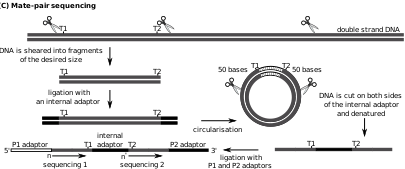
\includegraphics[width=\textwidth]{figures/mate-pairs-solid}
\end{frame}

\begin{frame}[fragile]
\frametitle{Shortest superstring}
\begin{block}{Istanza}
Insieme $\mathcal{S} = \{s_{1}, \ldots , s_{n}\}$ di stringhe
\end{block}
\begin{block}{Soluzioni ammissibili}
Superstring $T$ di $\mathcal{S}$.
Ogni $s_{i}$ è sottostringa di $T$
\end{block}

\begin{block}{Funzione obiettivo}
$|T|$
\end{block}

$T$ è il genoma assemblato, $\mathcal{S}$ le read

\begin{block}{Problema}
Regioni ripetute
\end{block}
\end{frame}

\begin{frame}[fragile]
\frametitle{TSP}
\end{frame}

\begin{frame}[fragile]
\frametitle{Overlay --- Layout --- Consensus}
\end{frame}

\begin{frame}[fragile]
\frametitle{Reverse and complement}
\end{frame}

\begin{frame}[fragile]
\frametitle{SBH}

Estrazione $k$-mers
\end{frame}


\begin{frame}[fragile]
\frametitle{Sequenziamento e grafi di de Brujin}
\end{frame}


%%% Local Variables:
%%% TeX-PDF-mode: t
%%% TeX-master: "graphs-video"
%%% buffer-file-coding-system: utf-8
%%% End:
